\documentclass[11pt]{article}
\usepackage[margin=2.4cm]{geometry}
\usepackage{graphicx}
\usepackage{booktabs}
\usepackage{tikz}
\usetikzlibrary{arrows.meta, positioning, shapes.geometric}
\usepackage{xcolor}
\usepackage{amsmath}
\usepackage{amssymb}
\usepackage[colorlinks=true, linkcolor=blue!60!black, urlcolor=blue!60!black]{hyperref}
\usepackage{caption}
\captionsetup{font=small, labelfont=bf}

\definecolor{envgreen}{HTML}{1b9e77}
\definecolor{envblue}{HTML}{3b6fb6}
\definecolor{warnred}{HTML}{b02418}
\newcommand{\ok}[1]{\textcolor{envgreen}{#1}}
\newcommand{\bad}[1]{\textcolor{warnred}{#1}}

\title{\textbf{The MemoryEnv T-maze}\\[2pt]
\large Environment, PPO agents, and the activation dataset --- working report}
\author{Crusoe-Cogniland}
\date{\today}

\begin{document}
\maketitle

\begin{abstract}
\noindent
MemoryEnv is a minimal T-maze for studying \emph{memory} in reinforcement-learning agents.
At the start of each episode the agent walks past a single \textbf{cue} carrying two independent
features --- a \textbf{direction} (up / down) and a \textbf{color} (green / blue). Long after the
cue has left its field of view, the agent must recall the direction to choose a branch at a fork,
and later recall the color to choose between two colored doors whose positions are randomized.
Three recurrent PPO agents were trained on nested subsets of the four possible cues (2cue / 3cue /
4cue); all three solve their training cues perfectly. This report documents the environment, the
map generation, the training setup and results, and the activation dataset that will be the basis
of the following interpretability experiments. Inconsistencies found while writing are collected
in Section~\ref{sec:issues}.
\end{abstract}

% ==================================================================
\section{The environment}

\subsection{Task structure}

Each episode is one corridor traversal with two memory-dependent decisions
(Figure~\ref{fig:schematic}):

\begin{enumerate}
  \item \textbf{Cue room.} The agent starts in a short corridor and passes through a small room
        containing one cue tile, drawn from
        $\{\text{green\_up},\ \text{blue\_up},\ \text{green\_down},\ \text{blue\_down}\}$
        (direction $\times$ color). The cue is visible only while the room is inside the agent's
        $5\times5$ view.
  \item \textbf{Fork (direction recall).} After a corridor, the maze splits around a thick central
        wall. The cue's \emph{direction} determines the rewarded branch: up-cues $\rightarrow$
        upper branch, down-cues $\rightarrow$ lower branch. Both branches reconnect.
  \item \textbf{Doors (color recall).} The corridor ends at a column with a green door and a blue
        door. Their vertical arrangement is randomized every episode (50/50), so the agent cannot
        memorize a side: it must recall the cue's \emph{color} and read the current door layout.
        Stepping on a door ends the episode; the correct door is the one matching the cue color.
\end{enumerate}

\begin{figure}[h]
\centering
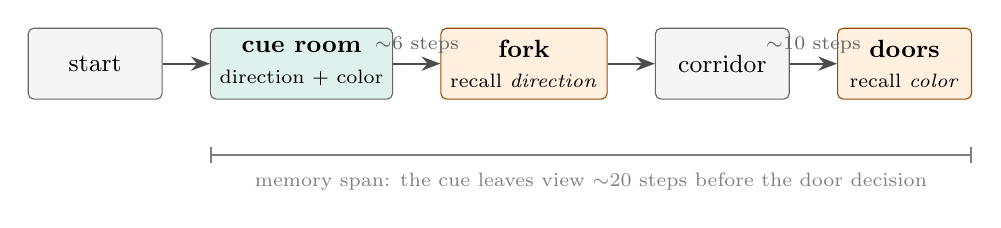
\begin{tikzpicture}[
  node distance=4mm and 6mm,
  box/.style={rectangle, rounded corners=2pt, draw=black!60, fill=black!4,
              minimum height=9mm, minimum width=17mm, align=center, font=\small},
  dec/.style={box, fill=orange!12, draw=orange!60!black},
  arr/.style={-{Stealth[length=2.4mm]}, thick, black!70}]
  \node[box] (start) {start};
  \node[box, right=of start, fill=envgreen!14] (cue) {\textbf{cue room}\\ \scriptsize direction + color};
  \node[dec, right=of cue] (fork) {\textbf{fork}\\ \scriptsize recall \emph{direction}};
  \node[box, right=of fork] (post) {corridor};
  \node[dec, right=of post] (door) {\textbf{doors}\\ \scriptsize recall \emph{color}};
  \draw[arr] (start) -- (cue);
  \draw[arr] (cue) -- node[above, font=\scriptsize, black!60]{$\sim$6 steps} (fork);
  \draw[arr] (fork) -- (post);
  \draw[arr] (post) -- node[above, font=\scriptsize, black!60]{$\sim$10 steps} (door);
  \draw[{Bar[width=2mm]}-{Bar[width=2mm]}, thick, black!50]
    ([yshift=-7mm]cue.south west) -- node[below=1mm, font=\scriptsize]
    {memory span: the cue leaves view $\sim$20 steps before the door decision}
    ([yshift=-7mm]door.south east);
\end{tikzpicture}
\caption{Episode structure. The two decisions test two independent bits held in memory:
direction $\rightarrow$ branch (unconditional mapping) and color $\rightarrow$ door
(\emph{conditional}: the recalled color must be matched against the randomized door layout).}
\label{fig:schematic}
\end{figure}

\begin{figure}[h]
\centering
\includegraphics[width=\textwidth]{env_maps.png}
\caption{Rendered maps for the four cue types (door layout green-top shown; red = optimal path).
Panel annotations state which models contain each cue in their training set.}
\label{fig:maps}
\end{figure}

\subsection{Map generation}

The maze geometry is \textbf{fixed and deterministic} --- there is no procedural map dataset and no
rotation or mirroring augmentation. \texttt{build\_geometry} computes all anchors from the config
(defaults in parentheses): pre-cue corridor (1 step + view margin), cue room ($4\times3$ cells),
pre-branch corridor (5), branch length (4), post-branch corridor (5), central wall thickness (3),
giving a $27 \times 9$ tile grid. Only three things are randomized per episode:
\begin{center}
\small
\begin{tabular}{lll}
\toprule
quantity & distribution & role \\
\midrule
cue type & uniform over the model's training set & the memory content \\
cue cell & uniform over room columns, upper/lower row & where the cue appears \\
door layout & green-top vs.\ blue-top, 50/50 & makes color recall conditional \\
\bottomrule
\end{tabular}
\end{center}

\noindent Two views of the same cue under both door layouts are shown in
Figure~\ref{fig:conditional}: the branch is fixed by the cue, but the correct door flips with the
layout.

\begin{figure}[h]
\centering
\includegraphics[width=\textwidth]{env_maps_conditional.png}
\caption{Same cue (green\_down), both door layouts. The rewarded branch (direction) is identical;
the rewarded door position flips --- the color memory must be combined with the observed layout.}
\label{fig:conditional}
\end{figure}

\subsection{Observation, actions, reward}

\textbf{Observation.} Symbolic and egocentric: a $5\times5$ crop of tile identities centred on the
agent (9 tile types: empty, wall, the 4 cue tiles, green door, blue door, out-of-bounds), one-hot
encoded ($5{\cdot}5{\cdot}9 = 225$ dims), concatenated with \textbf{5 scalars}:
\[
\text{scalars} \;=\; \big[\,
\underbrace{\mathbf{1}_{\text{East}},\ \mathbf{1}_{\text{South}},\ \mathbf{1}_{\text{West}},\ \mathbf{1}_{\text{North}}}_{\text{facing direction, one-hot}},\
\underbrace{t / T_{\max}}_{\text{episode progress} \in [0,1]}
\,\big]
\]
The facing one-hot is needed because the crop is \emph{axis-aligned}, not rotated with the agent:
the same view means different things depending on heading. The progress scalar is $t/200$.
Total flat dimension $225 + 5 = 230$. There is no compass and no position information beyond what
is visible in the crop.

\textbf{Actions.} Discrete(3), MiniGrid-style: turn left, turn right, move forward. Because
turning costs a step, the optimal episode is $\approx 34$ steps.

\textbf{Reward.} Sparse subgoals plus a small potential-based shaping on the agent's
$x$-progress:
\begin{align*}
r_t \;=\;& \underbrace{0.5\cdot\mathbf{1}[\text{entered direction-correct branch}]}_{\text{branch bonus}}
\;+\; \underbrace{0.5\cdot\mathbf{1}[\text{stepped on color-correct door}]}_{\text{success}} \\
&+\; \underbrace{0.01\,(\phi_t - \phi_{t-1})}_{\text{shaping}}
\;+\; \underbrace{p\cdot\mathbf{1}[\text{entered wrong branch}]}_{p \in \{0, -1\}\ \text{(per model, see \S\ref{sec:issues})}}
\end{align*}
Episodes terminate on any door (wrong door: 0 reward) or truncate at 200 steps. Maximum return
$\approx 1.23$ ($0.5 + 0.5 + $ shaping).

% ==================================================================
\section{Agents and training}

\subsection{Architecture: recurrent PPO (PPO+GRU)}

The agent is a single-file JAX implementation (\texttt{train\_ppo\_memory.py}). The observation is
embedded by a learned, shared per-tile embedding, passed through an MLP, and integrated over time
by a GRU --- the GRU hidden state is the agent's only memory. Actor and critic heads read the GRU
state (Figure~\ref{fig:arch}).

\begin{figure}[h]
\centering
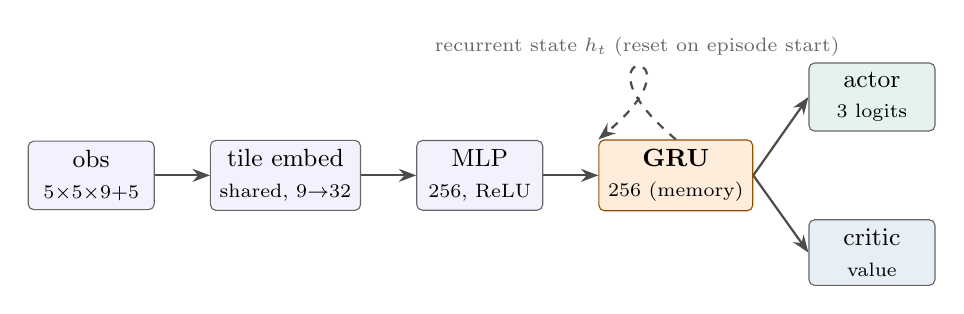
\begin{tikzpicture}[
  node distance=3.5mm and 7mm,
  blk/.style={rectangle, rounded corners=2pt, draw=black!60, fill=blue!5,
              minimum height=8mm, minimum width=16mm, align=center, font=\small},
  mem/.style={blk, fill=orange!14, draw=orange!60!black},
  arr/.style={-{Stealth[length=2.2mm]}, thick, black!70}]
  \node[blk] (obs) {obs\\ \scriptsize $5{\times}5{\times}9$+5};
  \node[blk, right=of obs] (emb) {tile embed\\ \scriptsize shared, $9{\to}32$};
  \node[blk, right=of emb] (mlp) {MLP\\ \scriptsize 256, ReLU};
  \node[mem, right=of mlp] (gru) {\textbf{GRU}\\ \scriptsize 256 (memory)};
  \node[blk, above right=1mm and 7mm of gru, fill=envgreen!12] (actor) {actor\\ \scriptsize 3 logits};
  \node[blk, below right=1mm and 7mm of gru, fill=envblue!12] (critic) {critic\\ \scriptsize value};
  \draw[arr] (obs) -- (emb); \draw[arr] (emb) -- (mlp); \draw[arr] (mlp) -- (gru);
  \draw[arr] (gru.east) -- (actor.west); \draw[arr] (gru.east) -- (critic.west);
  \draw[arr, dashed] (gru.north) to[out=140,in=40,looseness=5]
      node[above, font=\scriptsize, black!60]{recurrent state $h_t$ (reset on episode start)} (gru.north west);
\end{tikzpicture}
\caption{PPO+GRU architecture. All interpretability analyses operate on the 256-d GRU hidden
state $h_t$ (and, for comparison, the pre-GRU observation embedding).}
\label{fig:arch}
\end{figure}

\subsection{Training protocol}

Standard clipped PPO with GAE, trained end-to-end on real environment returns:
256 parallel environments $\times$ 128-step rollouts, 4 epochs $\times$ 8 minibatches per update
(minibatches split over environments, never over time, so the GRU sees unbroken sequences),
learning rate $2.5\times10^{-4}$ annealed linearly, $\gamma = 0.997$, $\lambda_{\text{GAE}} = 0.95$,
clip 0.2, value coefficient 0.5, gradient-norm clip 0.5, \textbf{25M} environment steps
($\approx$10 minutes on one RTX~3090 at $\approx$70k steps/s). Three models were trained on nested
cue sets:

\begin{center}
\small
\begin{tabular}{llccc}
\toprule
model & training cues & entropy coef. & wrong-branch penalty & seed \\
\midrule
2cue & green\_up, blue\_down & 0.03 & $-1.0$ & 1 \\
3cue & green\_up, green\_down, blue\_down & 0.01 & $-1.0$ & 0 \\
4cue & all four & 0.03 & $0.0$ & 1 \\
\bottomrule
\end{tabular}
\end{center}

\noindent\bad{Note the recipes are not uniform} --- each model is the survivor of its own tuning
sequence (details in \S\ref{sec:issues}). Exploration (entropy) and the wrong-branch penalty were
the two decisive knobs: 4cue only trained successfully after \emph{removing} the penalty.

\paragraph{Context: DreamerV3.} A carefully tuned DreamerV3 (25M and 50M parameters, several
reward variants, 8M steps) consistently solves the direction subgoal but leaves the color
$\rightarrow$ door subgoal at chance, even though probes show the color is perfectly represented
in its recurrent state. PPO on real returns solves both; this motivates the choice of the PPO
models as the substrate for the experiments that follow.

% ==================================================================
\section{Training results}

Evaluation: greedy policy, 96 episodes per cue type, random 50/50 door layouts
(\texttt{diag\_ppo.py}). ``Direction correct'' = took the branch matching the cue direction;
``success'' = ended on the color-correct door.

\begin{table}[h]
\centering
\small
\begin{tabular}{llcccc}
\toprule
model & cue & status & direction correct & success & \\
\midrule
2cue & green\_up   & trained  & \ok{1.00} & \ok{1.00} & \\
2cue & blue\_down  & trained  & \ok{1.00} & \ok{1.00} & \\
2cue & blue\_up    & held out & \bad{0.00} & 0.53 & \scriptsize generalizes by color, not direction \\
2cue & green\_down & held out & \bad{0.00} & 1.00 & \scriptsize (wrong branch, often right door) \\
\midrule
3cue & green\_up   & trained  & \ok{1.00} & \ok{1.00} & \\
3cue & green\_down & trained  & \ok{1.00} & \ok{1.00} & \\
3cue & blue\_down  & trained  & \ok{1.00} & \ok{1.00} & \\
3cue & blue\_up    & held out & \bad{0.00} & \bad{0.00} & \\
\midrule
4cue & all four    & trained  & \ok{1.00} & \ok{1.00} & \scriptsize return $1.230$ (max), ep.\ length $34.5$ \\
\bottomrule
\end{tabular}
\caption{Final evaluation. All models solve \emph{all their training cues} perfectly under
randomized doors. Held-out behaviour is systematic, not random: the 2cue model maps unseen cues by
their \emph{color} (blue $\rightarrow$ lower branch, green $\rightarrow$ upper), which is direction-wrong for
both held-out cues, yet it still often finds the color-correct door.}
\label{tab:results}
\end{table}

Figures~\ref{fig:traj2}--\ref{fig:traj4} show reference greedy trajectories on all four cues for
each model (both door layouts shown across panels; every panel is annotated trained / held out).

\begin{figure}[p]
\centering
\includegraphics[width=\textwidth]{traj_2cue.png}
\caption{2cue model, greedy trajectories. Trained cues are perfect; held-out cues take the
color-consistent (direction-wrong) branch.}
\label{fig:traj2}
\end{figure}
\begin{figure}[p]
\centering
\includegraphics[width=\textwidth]{traj_3cue.png}
\caption{3cue model, greedy trajectories.}
\label{fig:traj3}
\end{figure}
\begin{figure}[p]
\centering
\includegraphics[width=\textwidth]{traj_4cue.png}
\caption{4cue model, greedy trajectories: all four cues, both door layouts, all correct.}
\label{fig:traj4}
\end{figure}

% ==================================================================
\section{The activation dataset}
\label{sec:acts}

The dataset (\texttt{build\_ppo\_activations.py} $\rightarrow$
\texttt{outputs/ppo\_runs/<model>/activations.npz}) is the substrate for the probing and steering
experiments.

\paragraph{Collection protocol.} For each frozen model: \textbf{512 episodes}, greedy policy
(argmax actions), cues sampled \textbf{uniformly over all four types} (including cues the model
was not trained on), door layout randomized 50/50, episodes capped at \textbf{60 steps}
(optimal is $\approx$34). At every \emph{live} timestep (before the episode ends) we record:

\begin{center}
\small
\begin{tabular}{lll}
\toprule
field & shape & meaning \\
\midrule
\texttt{feat}       & $(N, 256)$ & GRU hidden state $h_t$ (post-update; what actor/critic read) \\
\texttt{obs\_embed} & $(N, 256)$ & encoder output (pre-GRU): current observation, no memory \\
\texttt{ep, t}      & $(N,)$     & episode index, timestep within episode \\
\texttt{cue\_type}  & $(N,)$     & 0..3 (green\_up, blue\_up, green\_down, blue\_down) \\
\texttt{shape}\footnotemark & $(N,)$ & cue \emph{direction} label (0 = up, 1 = down) \\
\texttt{colour}     & $(N,)$     & cue color label (0 = green, 1 = blue) \\
\texttt{phase}      & $(N,)$     & maze phase (pre-cue, cue-room, pre-branch, branch, post, door) \\
\texttt{cue\_vis}   & $(N,)$     & 1 iff a cue tile is inside the current $5\times5$ view \\
\texttt{action}     & $(N,)$     & greedy action taken \\
\texttt{agent\_x, agent\_y} & $(N,)$ & agent position (god's-eye) \\
\texttt{ep\_success} & $(N,)$    & episode-level outcome, repeated per step \\
\bottomrule
\end{tabular}
\end{center}
\footnotetext{Stored under the legacy key \texttt{shape}; throughout this report the feature is
called \emph{direction}.}

\paragraph{Sizes and composition.}
2cue: $18\,442$ rows; 3cue: $18\,606$; 4cue: $17\,648$ (rows differ because episodes end at
different times). Phases are all populated (e.g.\ 4cue: 2560 / 2048 / 4608 / 2048 / 4608 / 1776
steps for the six phases). Dataset-level \texttt{ep\_success} is 0.85 / 0.73 / 1.00 for
2 / 3 / 4cue --- below 1 for the smaller models \emph{only because held-out cues are included} in
the factorized sampling (cf.\ Table~\ref{tab:results}); on their trained cues all models are at
1.0.

\paragraph{Two representations.} \texttt{obs\_embed} encodes the \emph{current} observation only
--- cue information is present in it exclusively while the cue is in view. \texttt{feat} is the
recurrent memory: cue information appears when the cue is seen and \emph{persists} to the door.
Their contrast separates perception from memory in downstream analyses.

% ==================================================================
\section{The belief space: exact construction}
\label{sec:beliefspace}

All belief readouts and interventions operate on the \textbf{GRU hidden state}
$h_t \in \mathbb{R}^{256}$, using objects fit \emph{once, offline}, on the activation dataset of
Section~\ref{sec:acts} restricted to \textbf{training-set cues only} and to the post-cue phases
(\texttt{phase} $\geq$ pre-branch, i.e.\ the belief has been formed). Nothing is refit at run
time; real-time visualization is pure projection.

\paragraph{1. Cue-identity belief (the ``belief over time'' lines).} A multinomial logistic
regression is fit to predict the cue type $c$ from $h$ over the model's $K$ training cues
($K{=}2,3,4$):
\[
P(\text{cue}=c \mid h) \;=\; \mathrm{softmax}\big(W h + b\big)_c , \qquad W \in \mathbb{R}^{K\times 256}.
\]

\emph{Training data, exactly.} One sample per \emph{live timestep} of the activation-dataset
episodes, keeping only (i) episodes whose cue is in the model's training set and (ii) timesteps
in the post-cue phases (pre-branch onward), where the belief has been formed. The label of every
timestep is its episode's cue --- labels repeat within an episode. This yields
$N = 6478\,/\,10035\,/\,13040$ samples for the 2/3/4cue models, approximately class-balanced by
construction ($\approx$3000--3900 per cue; factorized sampling, no class weighting needed).
Features are the raw 256-d GRU states, \emph{not} standardized (they are tanh-bounded and share
scale).

\emph{Optimization, exactly.} sklearn \texttt{LogisticRegression(max\_iter=4000)}: multinomial
cross-entropy with the default L2 penalty ($C{=}1$), LBFGS solver, fitted intercept. The result
is the single weight matrix $W$ ($K \times 256$) and bias $b$ used everywhere afterwards ---
nothing is refit at run time.

\emph{The belief-over-time plot, exactly.} During any (greedy) episode, $h_t$ is the GRU state
\emph{after} processing observation $o_t$ --- the same tensor the actor reads. Each step plots the
$K$ values $\mathrm{softmax}(W h_t + b)$; the grey band marks steps where a cue tile is inside
the $5\times5$ view, the purple band marks intervention steps, and the dashed line is chance
$1/K$. Two caveats: (i) within-episode samples are temporally correlated, so the fit is a
readout, not an i.i.d.\ generalization claim --- but every curve shown is from a \emph{new}
rollout, out-of-sample by construction; (ii) the probe was trained on on-manifold post-cue
states, so its outputs on pre-cue steps (where it hovers near $1/K$) and on intervention-displaced
states are extrapolations.

\paragraph{2. Belief-plane axes.} Two binary logistic probes are fit on the same trained-only
samples: one for \emph{direction} (up/down), one for \emph{color} (green/blue); their
unit-normalized coefficient vectors $w_{\text{dir}}, w_{\text{col}}$ are the plane axes, and each
state is plotted at $\big(h_t \cdot w_{\text{dir}},\; h_t \cdot w_{\text{col}}\big)$.
\emph{Special case 2cue:} its two training cues confound direction with color, so the two probes
collapse onto one direction (cos $\approx$ 1) and no independent second axis exists. For that
model the plane instead uses $a_1 = (\mu_2 - \mu_1)/\lVert\cdot\rVert$ (the trained-cue
class-mean difference) and $a_2$ = the top principal component of the residual after projecting
$a_1$ out.

\paragraph{3. Landmarks and targets.} For each training cue $c$, the class mean
$\mu_c = \mathbb{E}[\,h \mid \text{cue}=c,\ \text{post-cue}\,]$ is ``the representation of cue
$c$ in memory''. The $\mu_c$ appear as landmarks in the plane and define the swap targets of
Section~\ref{sec:steer}. Axis limits are fixed from dataset percentiles, so the live point is
directly comparable across episodes.

\paragraph{Caveat.} These are \emph{decoding} objects: the best linear readout direction is not
guaranteed to be the causal direction the dynamics use --- and Section~\ref{sec:steer} shows both
directions of that mismatch empirically.

% ==================================================================
\section{Steering experiments}
\label{sec:steer}

Two interventions with opposite directions of causation, both on the GRU hidden state (no action
is ever replaced), evaluated with the greedy policy, $n{=}96$ episodes per condition, randomized
doors. Videos: \texttt{outputs/steer2\_\{2,3,4\}cue.mp4}.

\subsection{A. Steering behavior through activations, watching the belief}

At the fork (window $\mathcal{W}_A$: agent at the fork column, direction decision still open),
the hidden state is \textbf{minimally perturbed until the actor itself chooses the
direction-wrong action} $a^\star$ (supplied by a scripted navigator): iterating at most 15 times
with step $\eta = 0.25$,
\[
m(h) = \ell_{a^\star}(h) - \log\!\!\sum_{a \neq a^\star}\!\! e^{\ell_a(h)}, \qquad
h \leftarrow h + \eta\, \frac{\nabla_h m}{\lVert \nabla_h m \rVert} \quad \text{while } m(h) < 0,
\]
where $\ell(h)$ are the actor-head logits. The perturbed hidden is \emph{carried forward} by the
recurrence; the intervention ends at branch entry. A pure action-replacement control (override
$a_t$, never touch $h$) was also run for comparison.

\begin{table}[h]
\centering\small
\begin{tabular}{llcccc}
\toprule
model & cue & wrong branch & door correct & success & $P(\text{true cue})$ end (base) \\
\midrule
2cue & green\_up   & 1.00 & \ok{1.00} & \ok{1.00} & 1.00 (1.00) \\
2cue & blue\_down  & 1.00 & \ok{1.00} & \ok{1.00} & 0.70 (1.00) \\
3cue & green\_up   & 1.00 & \ok{1.00} & \ok{1.00} & 0.86 (1.00) \\
3cue & green\_down & 1.00 & 0.88 & 0.88 & 0.63 (1.00) \\
3cue & blue\_down  & 1.00 & \bad{0.67} & \bad{0.67} & 0.40 (1.00) \\
4cue & green\_up   & 1.00 & \ok{1.00} & \ok{1.00} & 0.70 (0.98) \\
4cue & blue\_up    & 1.00 & \bad{0.51} & \bad{0.51} & 0.77 (1.00) \\
4cue & green\_down & 1.00 & \ok{1.00} & \ok{1.00} & 0.78 (0.99) \\
4cue & blue\_down  & 1.00 & \ok{1.00} & \ok{1.00} & 1.00 (1.00) \\
\bottomrule
\end{tabular}
\caption{Experiment A. The activation push always achieves the wrong branch (efficacy 1.00). The
belief mostly survives and the agent recovers the color-correct door --- but, unlike the
action-replacement control (door correct $=1.00$ in \emph{all} nine conditions), the activation
edit \textbf{leaks}: door performance drops in 3/9 conditions and $P(\text{true cue})$ dips
broadly. A behavior-targeted activation edit is \emph{close to} but not exactly orthogonal to the
belief subspace.}
\label{tab:expA}
\end{table}

\subsection{B. Steering the belief transiently, watching the behavior}

Between the cue room and the direction decision only (window $\mathcal{W}_B$:
$x > x_{\text{room-end}}$ and branch undecided), the hidden is clamped along the axis between two
trained-cue representations,
\[
\hat u = \frac{\mu_{\text{tgt}} - \mu_{\text{src}}}{\lVert \mu_{\text{tgt}} - \mu_{\text{src}} \rVert},
\qquad
h \;\leftarrow\; h + \big(\mu_{\text{tgt}}\!\cdot\hat u \;-\; h\!\cdot\hat u\big)\,\hat u ,
\]
i.e.\ the coordinate along $\hat u$ is replaced by the target cue's typical value; all orthogonal
coordinates are untouched. \textbf{The clamp is released at branch entry} --- whatever drives the
door decision $\sim$15 steps later is the memory evolving freely.

\begin{table}[h]
\centering\small
\begin{tabular}{llcccc}
\toprule
model & swap (src $\rightarrow$ tgt) & branch as tgt & door as tgt & behaves as tgt & $P(\text{tgt})$ end \\
\midrule
2cue & green\_up $\rightarrow$ blue\_down & 1.00 & \bad{0.51} & \bad{0.51} & 0.47 \\
2cue & blue\_down $\rightarrow$ green\_up & 1.00 & 1.00 & \ok{1.00} & 1.00 \\
\midrule
3cue & green\_up $\rightarrow$ green\_down & 1.00 & 1.00 & \ok{1.00} & 1.00 \\
3cue & green\_up $\rightarrow$ blue\_down  & 1.00 & 1.00 & \ok{1.00} & 0.92 \\
3cue & green\_down $\rightarrow$ green\_up & \bad{0.00} & 1.00 & \bad{0.00} & 0.98 \\
3cue & green\_down $\rightarrow$ blue\_down & 1.00 & 1.00 & \ok{1.00} & 1.00 \\
3cue & blue\_down $\rightarrow$ green\_up  & 1.00 & 1.00 & \ok{1.00} & 1.00 \\
3cue & blue\_down $\rightarrow$ green\_down & 1.00 & 1.00 & \ok{1.00} & 1.00 \\
\midrule
4cue & green\_up $\rightarrow$ blue\_up    & 1.00 & 1.00 & \ok{1.00} & 1.00 \\
4cue & green\_up $\rightarrow$ green\_down & \bad{0.00} & 1.00 & \bad{0.00} & 1.00 \\
4cue & green\_up $\rightarrow$ blue\_down  & 1.00 & 1.00 & \ok{1.00} & 1.00 \\
4cue & blue\_up $\rightarrow$ green\_up    & 1.00 & 1.00 & \ok{1.00} & 0.97 \\
4cue & blue\_up $\rightarrow$ green\_down  & \bad{0.00} & 1.00 & \bad{0.00} & 1.00 \\
4cue & blue\_up $\rightarrow$ blue\_down   & 1.00 & 1.00 & \ok{1.00} & 1.00 \\
4cue & green\_down $\rightarrow$ green\_up & 0.80 & 1.00 & 0.80 & 1.00 \\
4cue & green\_down $\rightarrow$ blue\_up  & 1.00 & 1.00 & \ok{1.00} & 1.00 \\
4cue & green\_down $\rightarrow$ blue\_down & 1.00 & 1.00 & \ok{1.00} & 1.00 \\
4cue & blue\_down $\rightarrow$ green\_up  & 1.00 & 1.00 & \ok{1.00} & 0.95 \\
4cue & blue\_down $\rightarrow$ blue\_up   & 1.00 & 1.00 & \ok{1.00} & 1.00 \\
4cue & blue\_down $\rightarrow$ green\_down & 1.00 & 1.00 & \ok{1.00} & 0.91 \\
\bottomrule
\end{tabular}
\caption{Experiment B (transient swap, clamp released at branch entry). The implanted memory
\textbf{persists unaided} through the post-branch corridor and drives the door $\sim$15 steps
after release ($P(\text{tgt})$ end $\approx 1$) --- the belief state is self-sustaining. 17/20
swaps make the agent behave as the target cue end-to-end. Failures are structured: swaps
\emph{into green\_down} (and partially out of it) fail on the \emph{branch} while the probe
reports successful implantation --- the 1-D class-mean axis moves the readout but misses part of
the causal direction machinery. The transient clamp \emph{outperforms} a sustained one on 3cue
(sustained: door 0.50--0.61 on two pairs; transient: 1.00), indicating that releasing the state
lets the dynamics settle back onto the data manifold carrying the implanted belief.}
\label{tab:expB}
\end{table}

\subsection{Reading the results}

\begin{enumerate}
  \item \textbf{Behavior $\not\Rightarrow$ belief, mostly.} Forcing the wrong direction --- via
        actions (control: zero belief damage) or via minimal activation edits (small but real
        damage) --- leaves the agent able to recover and choose the color-correct door from the
        wrong branch. The belief content and the motor readout occupy largely separate directions
        of the same hidden vector.
  \item \textbf{Belief $\Rightarrow$ behavior, persistently.} A transient clamp before the fork
        implants a memory that survives on its own and controls both later decisions: a memory
        transplant, not a momentary bias.
  \item \textbf{Probe $\neq$ causal axis, in both directions.} Swaps into green\_down: probe says
        implanted, branch does not move. (In the earlier sustained-clamp run, blue\_down
        $\rightarrow$ green\_up behaved fully as target while the probe read only 0.28.)
        Direction appears to be encoded redundantly beyond the single class-mean axis; color is
        cleanly one-dimensional (color-involving swaps succeed everywhere).
\end{enumerate}

\begin{figure}[p]
\centering
\includegraphics[width=\textwidth]{steer2_2cue.png}
\caption{2cue model, same episode under the three conditions. Rows: trajectory (purple = steps
with the intervention active), cue-identity belief over time, belief-plane path. Note the
behavior-steered episode: belief lines barely move and the agent exits through the color-correct
door despite the forced wrong branch; the swapped episode jumps to the blue\_down landmark and
stays there after release.}
\label{fig:steer2a}
\end{figure}
\begin{figure}[p]
\centering
\includegraphics[width=\textwidth]{steer2_3cue.png}
\caption{3cue model, same layout.}
\label{fig:steer2b}
\end{figure}
\begin{figure}[p]
\centering
\includegraphics[width=\textwidth]{steer2_4cue.png}
\caption{4cue model, same layout. In the behavior-steered episode the belief dips
\emph{during} the activation push and recovers after release --- the ``leak'' of
Table~\ref{tab:expA}, visible in time.}
\label{fig:steer2c}
\end{figure}

% ==================================================================
\section{Inconsistencies and caveats found during write-up}
\label{sec:issues}

\begin{enumerate}
  \item \textbf{Non-uniform training recipes.} The three released models differ in entropy
        coefficient (0.03 / 0.01 / 0.03) and wrong-branch penalty ($-1$ / $-1$ / $0$), and were
        selected as the survivors of separate tuning attempts (PPO showed strong seed sensitivity:
        several configurations collapsed to a never-terminating shaping optimum). Cross-model
        comparisons therefore compare \emph{tasks + recipes}, not tasks alone. A controlled rerun
        (one recipe, several seeds per cue set) would clean this up.
  \item \textbf{Seed was not persisted.} \texttt{config.json} did not store the seed (recovered
        from the launch scripts: 1 / 0 / 1). Fixed in \texttt{train\_ppo\_memory.py} for future
        runs.
  \item \textbf{Held-out cues are inside the activation dataset.} Sampling is uniform over all
        four cues for every model. This is intentional (it lets us study generalization), but any
        probe fit on the full dataset for the 2cue/3cue models mixes on- and off-distribution
        states; analyses must condition on trained cues where appropriate.
  \item \textbf{Episode cap at 60 steps} during collection (vs.\ 200 in evaluation): held-out-cue
        episodes that wander can be truncated without reaching a door; \texttt{ep\_success}
        conflates ``wrong door'' and ``no door''. Not an issue for trained cues
        ($\approx$34-step episodes).
  \item \textbf{Legacy field name.} The direction label is stored as \texttt{shape} in the
        \texttt{.npz} files; renaming would break existing scripts, so the alias is documented
        here instead.
  \item \textbf{2cue held-out branch behaviour is anti-correlated} (direction correct $= 0.00$,
        not $0.5$): the model routes unseen cues by color. This is a property of its entangled
        code and must not be read as noise.
\end{enumerate}

\vspace{2mm}
\noindent\textit{Further experiments (belief geometry across models, input-level counterfactuals,
multi-dimensional swap axes for the direction anomaly) will be added incrementally.}

\end{document}
